\documentclass{beamer}
\usepackage[utf8]{inputenc}
\usepackage{amssymb}
\usepackage{pifont}
\usepackage{xcolor}
\usepackage{bigints}
\usepackage{mathrsfs}
\definecolor{dgreen}{rgb}{0.,0.6,0.}
\newcommand{\cmark}{{\color{dgreen}\ding{51}}}%
\newcommand{\xmark}{{\color{red}\ding{55}}}%
\newcommand{\bmark}{{\color{orange}$\sim$}}%

\usetheme{Dresden}
\usecolortheme{dolphin}
%\useoutertheme{infolines}

\beamertemplatenavigationsymbolsempty
\setbeamerfont{page number in head/foot}{size=\large}
\setbeamertemplate{footline}[frame number]

\addtobeamertemplate{navigation symbols}{}{%
    \usebeamerfont{footline}%
    \usebeamercolor[fg]{footline}%
    \hspace{1em}%
    \insertframenumber/\inserttotalframenumber
}
\setbeamercolor{footline}{fg=blue}


%for backup slides
\newcommand{\backupbegin}{
   \newcounter{finalframe}
   \setcounter{finalframe}{\value{framenumber}}
}
\newcommand{\backupend}{
   \setcounter{framenumber}{\value{finalframe}}
}

%\AtBeginSection[
%  {\frame<beamer>{\frametitle{Outline}   
%    \tableofcontents[currentsection,currentsubsection]}}%
%]%
%{
%  \frame<beamer>{ 
%    \frametitle{Outline}   
%    \tableofcontents[currentsection,currentsubsection]}
%}
\AtBeginSection[
  {\frame<beamer>{\frametitle{Outline}   
    \tableofcontents[currentsection,currentsection]}}%
]%
{
  \frame<beamer>{ 
    \frametitle{Outline}   
    \tableofcontents[currentsection,currentsection]}
}

\defbeamertemplate*{title page}{customized}[1][]
{
  \vfill
  \usebeamerfont{title}\inserttitle\par
  \usebeamerfont{subtitle}\usebeamercolor[fg]{subtitle}\insertsubtitle\par
  \bigskip
  \hfill\usebeamerfont{author}\insertauthor\par
  \hfill\textcolor{black}{Encadré par~: Anaïs Crestetto\\\hfill et Nicolas Crouseilles}\par
  \vfill
  \hfill\usebeamerfont{date}\insertdate\par
}


\title[]{Hybrid fluid/kinetic modeling for plasma}
\subtitle{WENO method for plasma simulation}
\author{Josselin Massot}
\date{2018/12/10}


\begin{document}

  \begin{frame}[plain,t]
    \titlepage
  \end{frame}

  \begin{frame}{What is plasma or rarefied gas ?}
    \begin{itemize}
      \item System of interacting particles
      \item Plasma : hot gas, electrons separated from atoms $\rightarrow$ electric field
      \item Examples of plasmas~:
        \begin{itemize}
          \item neons, ITER, nebula
        \end{itemize}
      \item Examples of rarefied gas~:
        \begin{itemize}
          \item atmospheric entry (Soyouz, CST-100 Starliner, \dots)
        \end{itemize}
    \end{itemize}
    \ \hfill 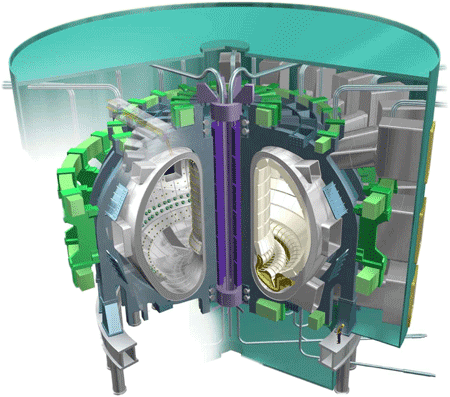
\includegraphics[height=0.3\textheight]{img/tokamak.png} \hfill 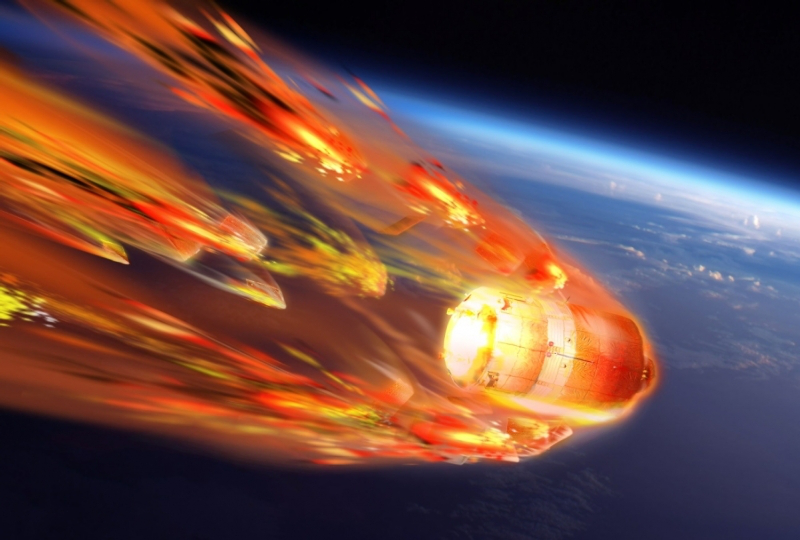
\includegraphics[height=0.3\textheight]{img/space.png} \hfill \ 
  \end{frame}


  \begin{frame}
    \tableofcontents
  \end{frame}

  \section{Models}
  \begin{frame}{Models}
  	\begin{description}
      \item[Microscopic model:] simulation of all particles \\
          $(t,x_i(t),v_i(t)), i=1,\dots,N$ \\
          \cmark{} accuracy $\quad$ \xmark{} computational time and memory
      \item[Macroscopic model:] plasma $\approx$ fluid \\
          $(\rho,u,T)(t,x)$ thermodynamic variables \\
          \xmark{} accuracy $\quad$ \cmark{} computational time and memory
      \item[Kinetic model:] simulation in phase space \\
          $f(t,x,v)$ distribution of density in phase space \\
          \bmark{} accuracy $\quad$ \bmark{} computational time and memory
    \end{description}
    Study only on macroscopic and kinetic models
  \end{frame}


  \subsection{Classical models}
  \begin{frame}{Macroscopic model}
    Euler's equations:

    $$
      \partial_t U + \nabla_x\cdot\mathcal{F}(U) = S_E(U)
    $$

    \begin{itemize}
      \item $U = U(t,x)$
      \item Vector $U = (\rho,\rho u,e)^{\textsf{T}}$ thermodynamic variables
      \item $S_E(U)$ source term that includes electric field $E$
    \end{itemize}
  \end{frame}

  \begin{frame}{Kinetic model}
    Vlasov-BGK's equation:
    $$
      \partial_t f + v\cdot\nabla_x f + E\cdot\nabla_v f = \frac{1}{\varepsilon}Q(f,f)
    $$

    Transport $(x,v)$ + stiff term $\frac{1}{\varepsilon}$

    \begin{itemize}
      \item $f = f(t,x,v)$ density distribution in phase space
      \item $Q(f,f)$ collision operator (BGK) $Q(f,f) = \mathcal{M}_{[U]}-f$
      \item $\mathcal{M}_{[U]}$: velocity distribution at equilibrium
      \item $\varepsilon$ $\sim$ mean free path \begin{itemize}
	      \item If $\varepsilon \ll 1$ $\rightarrow$ Euler equations
	      \item If $\varepsilon \gg 1$ $\rightarrow$ no collision (what I do now)
	     \end{itemize}
    \end{itemize}

    Relation with macroscopic variables:
    $$
      \bigintsss_{\mathbb{R}^d} \begin{pmatrix}1 \\ v \\ |v|^2 \end{pmatrix}f(t,x,v)\,\mathrm{d}v =
      \bigintsss_{\mathbb{R}^d} \begin{pmatrix}1 \\ v \\ |v|^2 \end{pmatrix}\mathcal{M}_{[U]}(t,x,v)\,\mathrm{d}v
      = U(t,x)
    $$
  \end{frame}

  \begin{frame}{Electric field}
    Poisson's equation

    $$
      \nabla_x\cdot E (x) = \rho (t,x) = \int_{\mathbb{R}^d} f(t,x,v)\,\mathrm{d}v
    $$

    Periodic conditions in space: resolution by FFT

    Maxwell's equation (magnetic field) soon! (one day)
  \end{frame}

  \subsection{Hybrid model}
  \begin{frame}{Hybrid model}
    \begin{enumerate}
      \item Micro-macro model (\textbf{mM})
        $$
          f = \underbrace{\mathcal{M}_{[U]}}_{\text{thermodynamic equilibrium state}} + \underbrace{g_{\phantom{[U]}}}_{\text{gap from equilibrium}}
        $$
      \item Approximation of \emph{micro} part (\textbf{mMh}) without interface between models (internship work)
        \begin{itemize}
          \item Transition function $h(t,x)$ between fluid area $\Omega_F$ and kinetic area $\Omega_K$
        \end{itemize}
    \end{enumerate}
  \end{frame}

  \begin{frame}{Building hybrid model}
    \begin{columns}
        \hspace*{0cm}
      \begin{column}{1.1\textwidth}
        \begin{enumerate}
          \setcounter{enumi}{0}
          \item \textbf{mM} consisting of 2 equations:
            \begin{description}
              \item[macro:] \textbf{mean} in $v$ of kinetic model:
              $$
                \partial_t U + \nabla_x\cdot\mathcal{F}(U) + {\color{dgreen}\nabla_x\cdot\langle vm(v)g \rangle_v} = S_E(U)
              $$

              \item[micro:] \textbf{projection} of kinetic model on image of collision operator $Q(f,f) = \mathcal{M}_{[U]} - f$:
              $$
                \partial_t g + (I-\Pi)[ v\cdot\nabla_x ({\color{dgreen}\mathcal{M}_{[U]}}+g) + E\cdot\nabla_v ({\color{dgreen}\mathcal{M}_{[U]}}+g) ] = -\frac{1}{\varepsilon}g
              $$
            \end{description}

            \textbf{mM} model is equivalent to kinetic model
        \end{enumerate}
      \end{column}
    \end{columns}
  \end{frame}

  \begin{frame}{Approximation of \emph{micro} part}
    \begin{columns}
        \hspace*{0cm}
      \begin{column}{1.1\textwidth}
        \begin{enumerate}
          \setcounter{enumi}{1}
          \item \textbf{Hypothesis:} $f = \mathcal{M}_{[U]}$ on $\Omega_F$ $\Rightarrow$ $g_F = 0$

            \textbf{New model:} approximation of \textbf{micro}-macro by domain decomposition
            $$
              \Omega = \Omega_F \cup \Omega_K \qquad g = {\color{red}(1-h)g} + {\color{blue}hg} = {\color{red}g_F} + {\color{blue}g_K}
            $$

            \begin{figure}
              \centering
              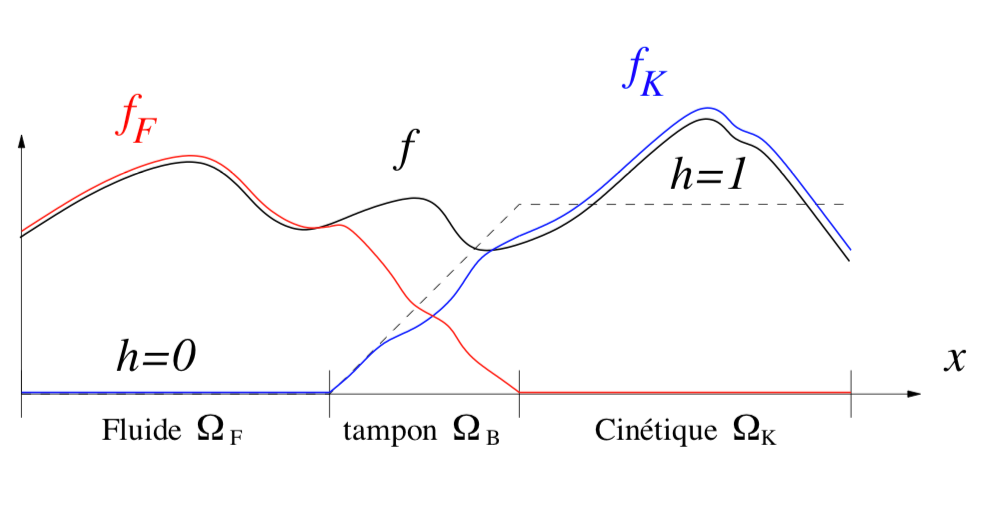
\includegraphics[height=0.4\textheight]{img/hx.png}
            \end{figure}
        \end{enumerate}
      \end{column}
    \end{columns}  
  \end{frame}

  \begin{frame}{Approximated \emph{micro} part}
    We multiply by $h$ micro part to get:

    $$
      \begin{aligned}
        \partial_t g_{\color{dgreen}K} + (I-\Pi)\left[ v\cdot\nabla_x (\mathcal{M}_{[U]}+g_{\color{dgreen}K}) \right.&+\left. E\cdot\nabla_v (\mathcal{M}_{[U]}+g_{\color{dgreen}K}) \right] = \\
                                                                                      &-\frac{1}{\varepsilon}g_{\color{dgreen}K} + {\color{dgreen}\frac{g_K}{h}\partial_t h}
      \end{aligned}
    $$

    Outside the support of $h$: $g_K = 0$

    \ 

    \textbf{Why this model?} save computational time (kinetic evaluation \textbf{only} on $\Omega_K$)
  \end{frame}

  %%%%%%%%%%%%%%%%%%%%%%%%%%
  \section{Schemes}
	\begin{frame}{Goals}
		\begin{itemize}
      \item Transport in phase space $(x,v)$                               $\rightsquigarrow$ scheme easy to use in multi-$d$ ($d$ at least 2)
      \item Heavy gradient                                                 $\rightsquigarrow$ need high order scheme
      \item Stiff term in $\frac{1}{\varepsilon}$, $\varepsilon \in ]0,1]$ $\rightsquigarrow$ need adapted time integrators
      \item Long time simulation                                           $\rightsquigarrow$ need stability of space+time scheme
		\end{itemize}
	\end{frame}

  \subsection{Time discretization}
  \begin{frame}{Explicit Euler method}

    Unstable with 5\textsuperscript{th}-order WENO method:\begin{itemize}\item {[Wang, R., \& Spiteri, R. (2007) SINUM]}\end{itemize}


    Amplification term is small enough to be \emph{controlled} by {\tiny very} small $\Delta t$.

    If stiff term $\rightsquigarrow$ IMEX:

    $$
      f^{n+1} = f^n -dt(v\partial_x+E\partial_v)(f^n) + \frac{1}{\varepsilon}(\mathcal{M}_{[U^{{\color{red}n+1}}]}-f^{{\color{red}n+1}})
    $$

    CFL upwind-IMEX: $\frac{\Delta x}{v_{\text{max}}}$

  \end{frame}
  \begin{frame}{Runge-Kutta 3th order method}
    Stable with 5\textsuperscript{th}-order WENO method (see later)

    If stiff term $\rightsquigarrow$ exponential formulation:

    $$
      \partial_t(e^{\frac{t}{\varepsilon}}g) + (I-\Pi)\left((v\partial_x+E\partial_v)(e^{\frac{t}{\varepsilon}}(g+\mathcal{M}_{[U]}))\right) = 0
    $$

    and Lawson scheme or IFRK method
  \end{frame}

  \subsection{Space discretization}
\begin{frame}{Compact scheme}
    \begin{figure}
      \centering
      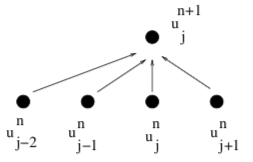
\includegraphics[height=0.4\textheight]{img/carac.png}
    \end{figure}
    \begin{itemize}
      \item High order 6 points scheme $(u^n_{j-3},\dots,u^n_{j-2})$
      \item Based on \textbf{1} polynomial of degree 5
    \end{itemize}
    It doesn't work very well (implementation bug ?) and it oscillates with discontinuity (not important for us) or heavy gradient (strong problem for filamentation).
  \end{frame}

  \begin{frame}{Numerical order}
    \begin{columns}[c]
      \column{.6\textwidth}
        $$
          \partial_t u + \partial_x u = 0
        $$

        initial: $u(t=0,x) = cos(x)$\\
        solution: $u(t=t_i,x) = cos(x-t_i)$ 

        \ 

        \begin{tabular}{c|c|c}
          $\Delta x$       & $\Delta t$        & $T_f$ \\
          \hline
          $\frac{2\pi}{N}$ & $10^{-5}\Delta x$ & $1$ \\
        \end{tabular}

        \ 

        $ N = 10, \dots , 200$

      \column{.5\textwidth}
        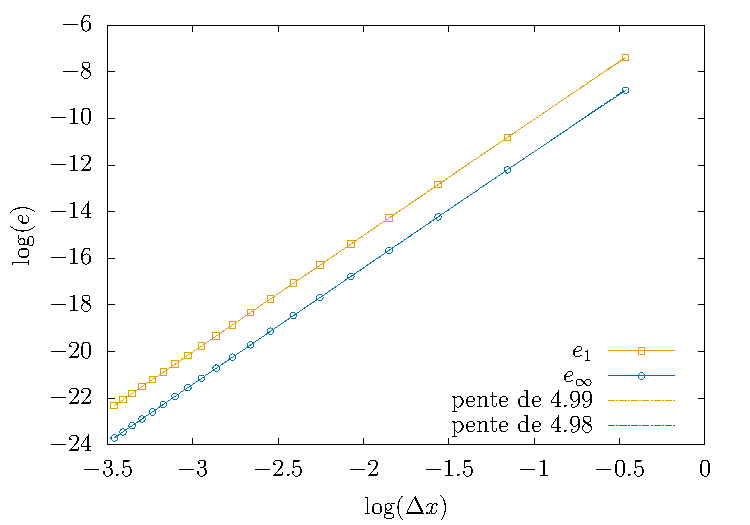
\includegraphics[width=\textwidth]{img/ordre_compact.pdf}
    \end{columns}
  \end{frame}

  \begin{frame}{Simplest test}
    Transport in 1 direction of a discontinuity
    \begin{columns}[c]
      \column{0.5\textwidth}
        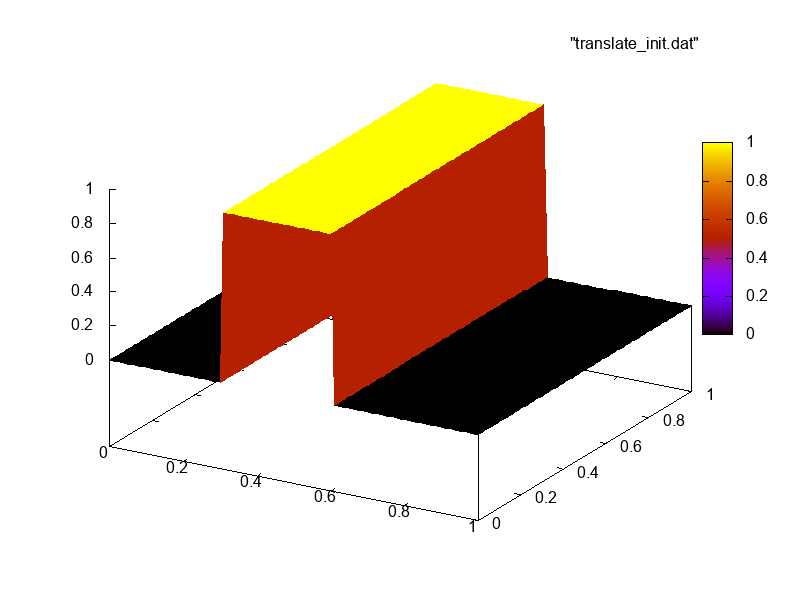
\includegraphics[width=\textwidth]{img/creneau_ci.png}

        Initial condition
      \column{0.5\textwidth}
        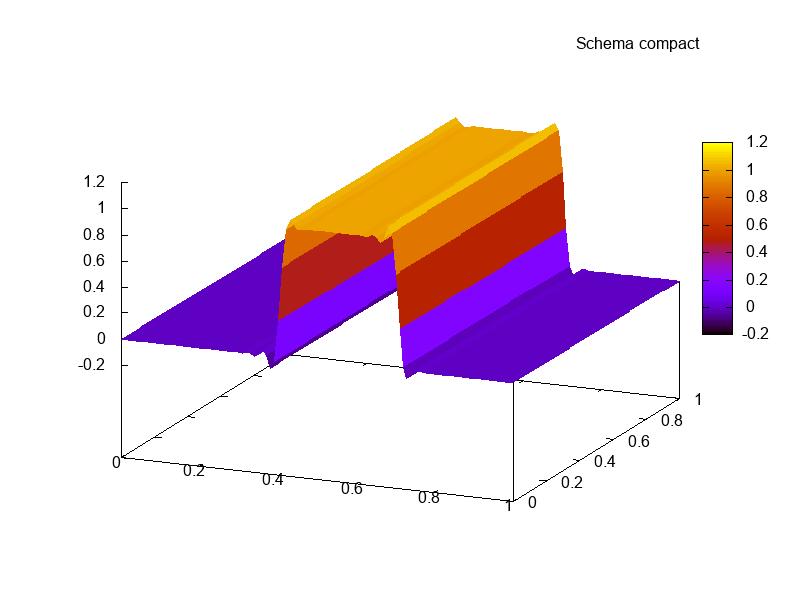
\includegraphics[width=\textwidth]{img/creneau_compact.png}

        Result
    \end{columns}
  \end{frame}

\begin{frame}{WENO method}
    \begin{itemize}
      \item High order 6 points scheme
      \item Based on \textbf{3} ENO approximations (of lower order) combined with non-linear weights (indicator of smoothness)
    \end{itemize}
    \textbf{BUT:} Unstable with explicit Euler method [Wang, R., \& Spiteri, R. (2007) SINUM]
  \end{frame}

  \begin{frame}{Numerical order}
    \begin{columns}[c]
      \column{.6\textwidth}
        $$
          \partial_t u + \partial_x u = 0
        $$

        initial: $u(t=0,x) = cos(x)$\\
        solution: $u(t=t_i,x) = cos(x-t_i)$ 

        \ 

        \begin{tabular}{c|c|c}
          $\Delta x$       & $\Delta t$        & $T_f$ \\
          \hline
          $\frac{2\pi}{N}$ & $10^{-5}\Delta x$ & $1$ \\
        \end{tabular}

        \ 

        $ N = 10, \dots , 200$
      \column{.5\textwidth}
        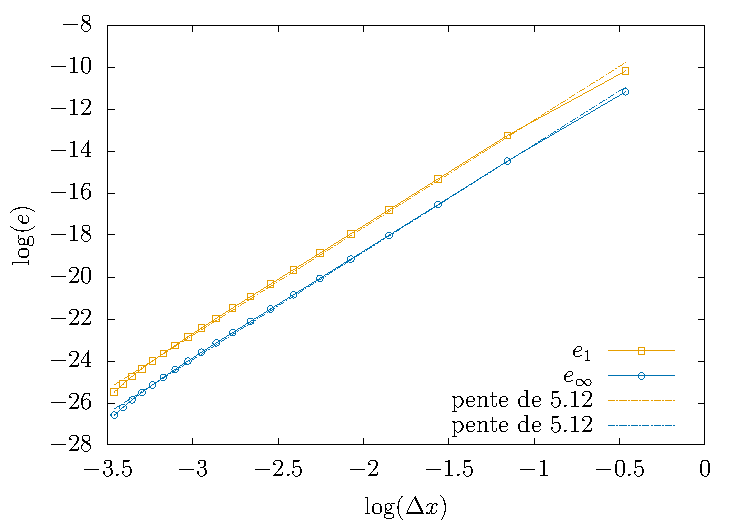
\includegraphics[width=\textwidth]{img/ordre_weno.pdf}
    \end{columns}
  \end{frame}

  \begin{frame}{Simplest test}
    Transport in 1 direction of a discontinuity
    \begin{columns}[c]
      \column{0.5\textwidth}
        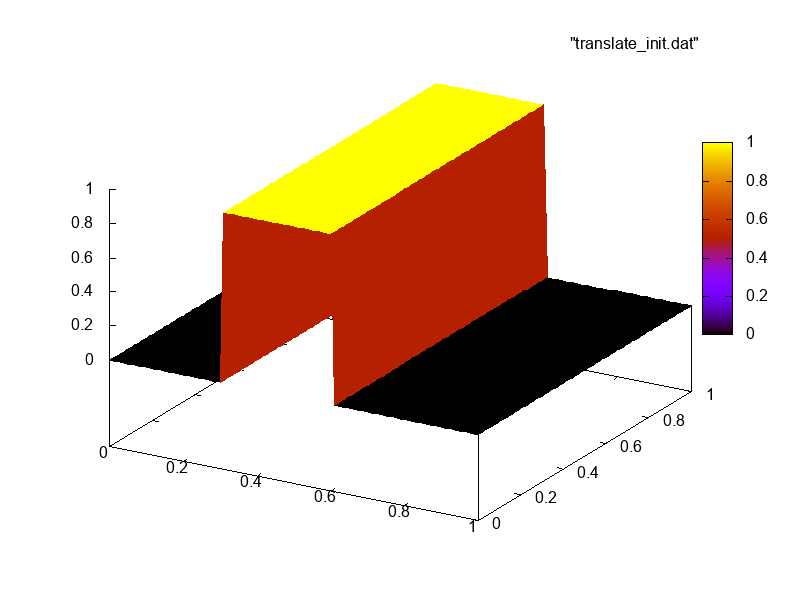
\includegraphics[width=\textwidth]{img/creneau_ci.png}

        Initial condition
      \column{0.5\textwidth}
        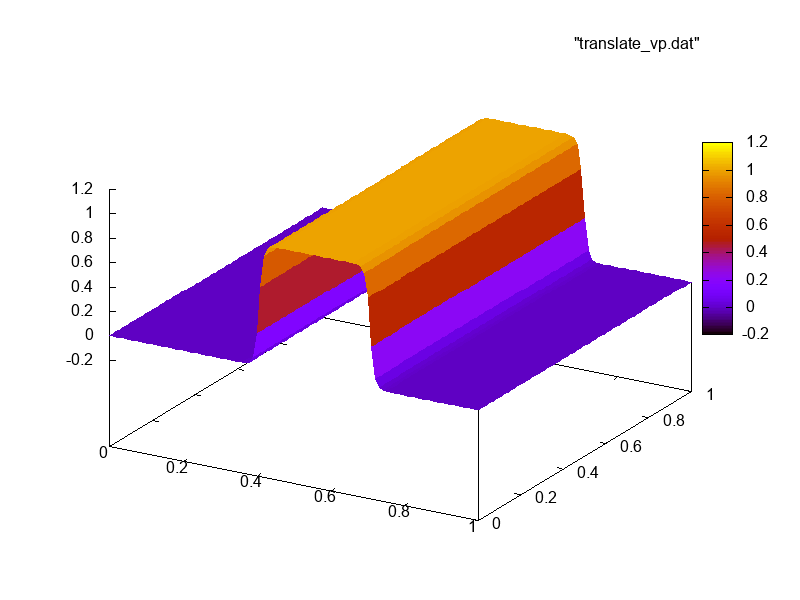
\includegraphics[width=\textwidth]{img/creneau_weno.png}

        Result
    \end{columns}
  \end{frame}

  \begin{frame}{Instability illustration}
    Gaussian rotation
    \begin{columns}[c]
      \column{0.5\textwidth}
        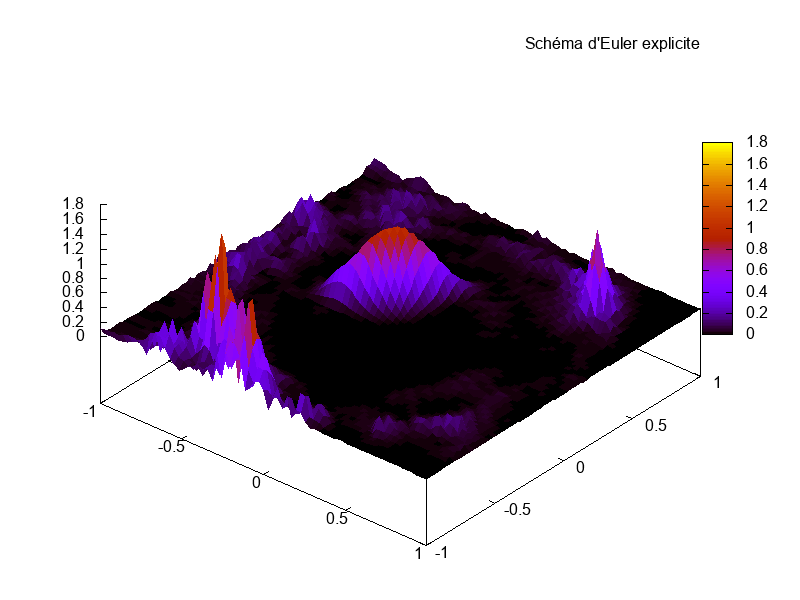
\includegraphics[width=\textwidth]{img/rotation_euler.png}

        Explicit Euler method
      \column{0.5\textwidth}
        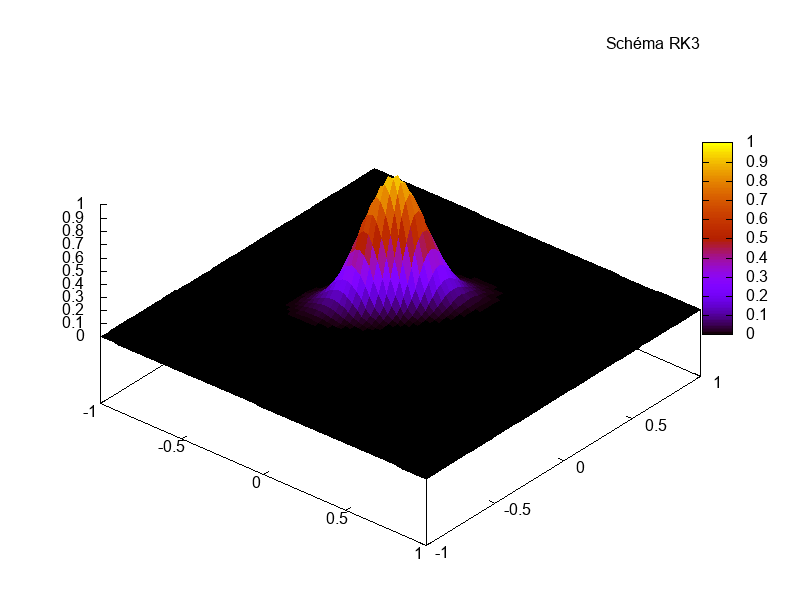
\includegraphics[width=\textwidth]{img/rotation_rk3.png}

        RK3 method
    \end{columns}

    \ 

    grid: $100\times 100$ \hfill $\Delta t = 0.3\Delta x$ \hfill $T_f = 15$ \\

    [Wang, R., \& Spiteri, R. (2007) SINUM]
  \end{frame}

  \begin{frame}{Steps of proof of instability}

    \begin{enumerate}
      \item Von Neumann analysis : $f_{j+k}^n \rightarrow e^{ik\phi}$ ($\phi \equiv \kappa\pi\Delta x$)
      \item Linearized WENO scheme (weight $\approx$ $\mathcal{O}(\Delta x^2)$):

        $$
          z(\phi) = \tilde{z}(\phi) + M(\epsilon_i,\phi)
        $$

        with $M(\epsilon_i,\phi) = \mathcal{O}(\Delta x^2)$
      \item Draw $\tilde{z}(\phi)$ with some RK stability curve and conclude.
    \end{enumerate}
  \end{frame}

  \begin{frame}{Stability of RK$N$-WENO}
  	\only<1>{
  		RK1-WENO
      \begin{figure}
        \centering
        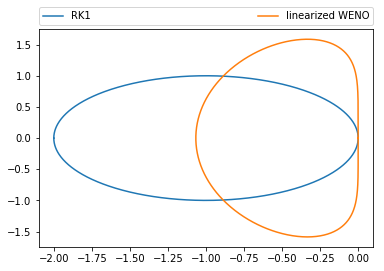
\includegraphics[height=0.65\textheight]{img/rk1-weno.png}
      \end{figure}
  	}
  	\only<2>{
  		RK2-WENO
      \begin{figure}
        \centering
        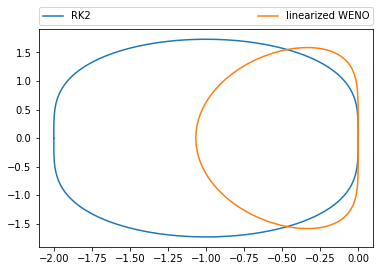
\includegraphics[height=0.65\textheight]{img/rk2-weno.png}
      \end{figure}
      possible stability: $\Delta t = 1.73\Delta x^{5/3}$ [Motamed, M., \& Macdonald, C. \& Ruuth S. (2010) J. Sci. Comput.]
  	}
  	\only<3>{
  		RK3-WENO (CFL: 1.433)
      \begin{figure}
        \centering
        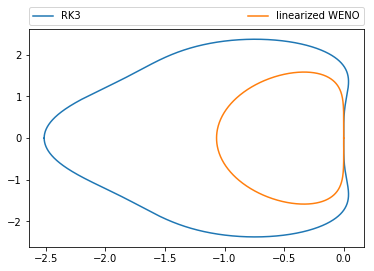
\includegraphics[height=0.65\textheight]{img/rk3-weno.png}
      \end{figure}
  	}
  	\only<4>{
  		RK4-WENO (CFL: 1.731)
      \begin{figure}
        \centering
        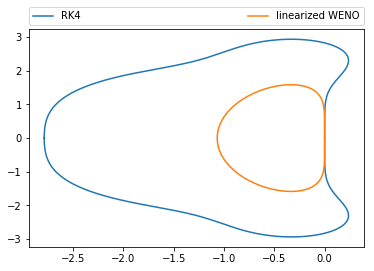
\includegraphics[height=0.65\textheight]{img/rk4-weno.png}
      \end{figure}
  	}
  \end{frame}

  %%%%%%%%%%%%%%%%%%%%%%%%%%
  \section{Numerical test}
  \subsection{Validation tests}
  \begin{frame}{Sod shock tube}
  	\textbf{Fluid regime validation} \\

    boundary: Neumann in space $x$, periodic in velocity $v$ \\
    initial condition: discontinuity in $\rho$ and $T$:
    $$
      U(t=0,x) = \begin{cases}
        U_L = (\rho_L,u_L,T_L) = (1,0,1) &, x \leq \frac{1}{2} \\
        U_R = (\rho_R,u_R,T_R) = (0.125,0,0.8)              &, x > \frac{1}{2}
      \end{cases}
    $$

    $$
      f(t=0,x,v) = \mathcal{M}_{[U(t=0,x)]}(x,v) \qquad g(t=0,x,v) = 0
    $$
  \end{frame}

  \begin{frame}{Models and schemes validation}
    \only<1>{
      $\rho(t=0.067,x)$
      \begin{figure}
        \centering
        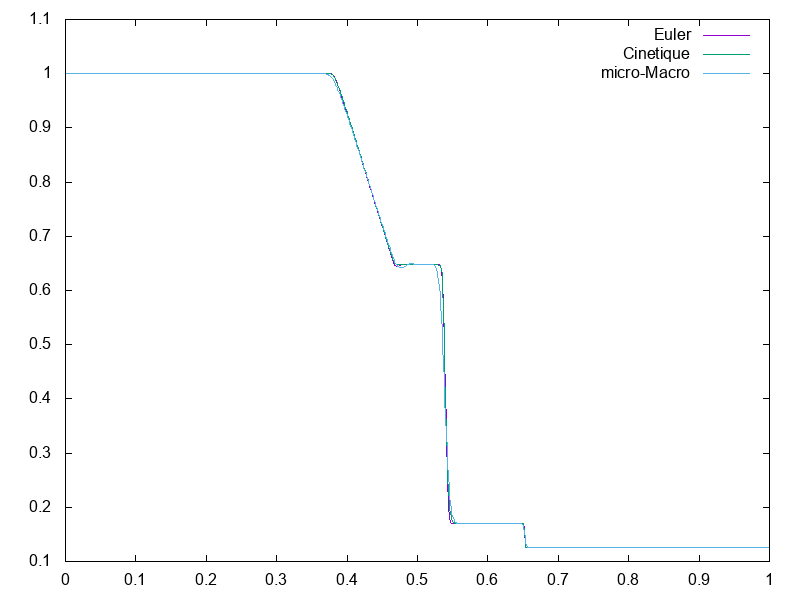
\includegraphics[height=0.55\textheight]{img/neu_rho.png}
      \end{figure}
    }
    \only<2>{
      $u(t=0.067,x)$
      \begin{figure}
        \centering
        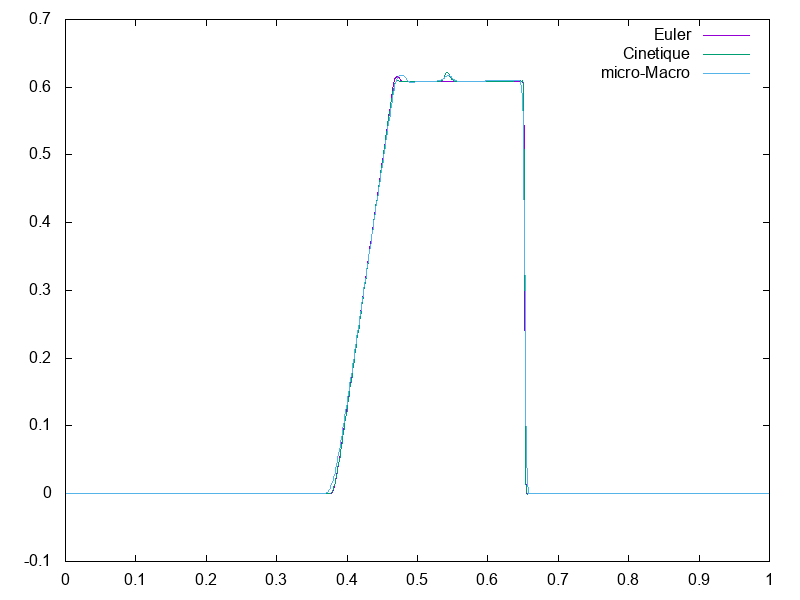
\includegraphics[height=0.55\textheight]{img/neu_u.png}
      \end{figure}
    }
    \only<3>{
      $T(t=0.067,x)$
      \begin{figure}
        \centering
        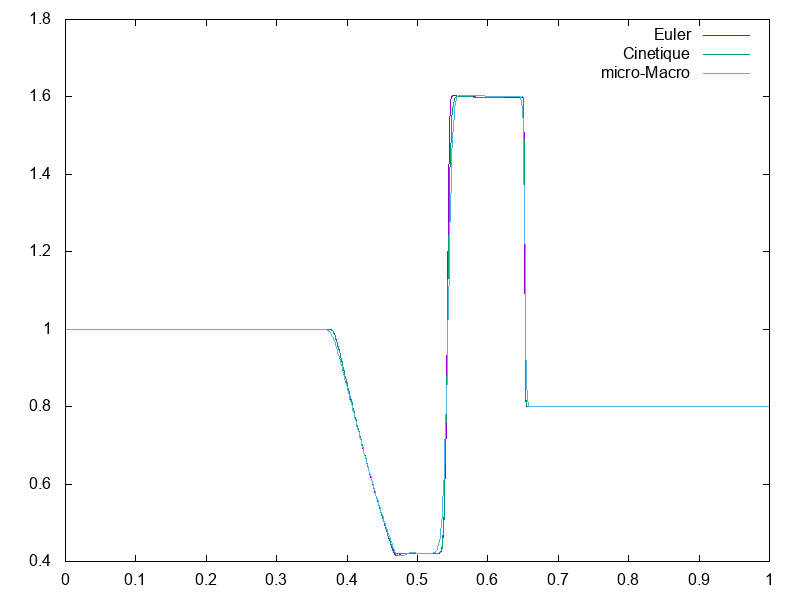
\includegraphics[height=0.55\textheight]{img/neu_T.png}
      \end{figure}
    }
    domain: $[0,1]\times[-18,18]$ \hfill grid: $1000\times 64$ \hfill $\varepsilon = 10^{-4}$ \\
    $\Delta x = 10^{-3}$            \hfill $\Delta v = 0.5625$       \hfill $\Delta t = \frac{1}{2}\frac{\Delta x}{v_{\text{max}}} = 2.77\cdot 10^{-5}$
  \end{frame}
  \begin{frame}{Simulation : Sod shock tube, kinetic mode: $\varepsilon = 1$}
    \begin{figure}
      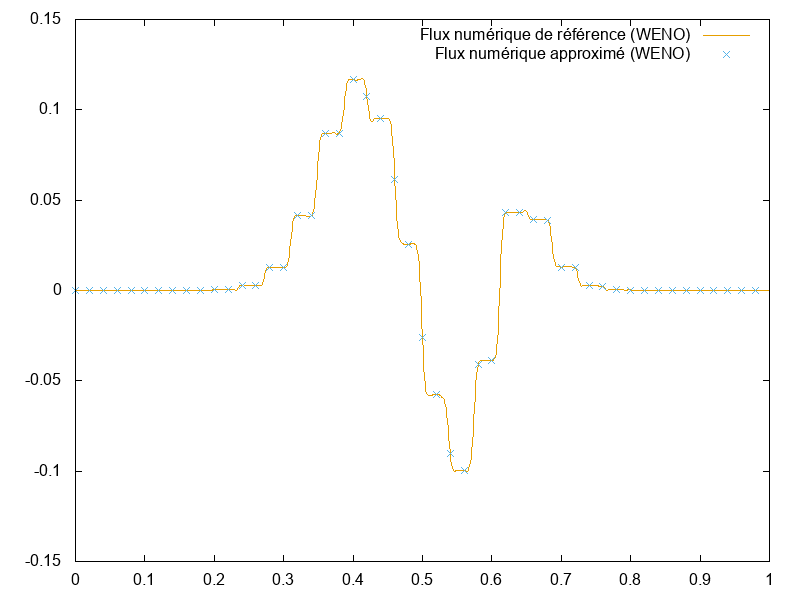
\includegraphics[height=0.55\textheight]{img/h/neuh_4_g.png}
    \end{figure}
    domain: $[0,1]\times[-18,18]$ \hfill grid: $1000\times 64$ \hfill $\varepsilon = 1$ \\
    $\Delta x = 10^{-3}$            \hfill $\Delta v = 0.5625$       \hfill $\Delta t = \frac{1}{2}\frac{\Delta x}{v_{\text{max}}} = 2.77\cdot 10^{-5}$ \\
    \textbf{Computing time:} divided by 2
  \end{frame}

  \begin{frame}{Numerical test: two streams}
		\begin{columns}[c]
      \column{0.5\textwidth}
      	\centering
        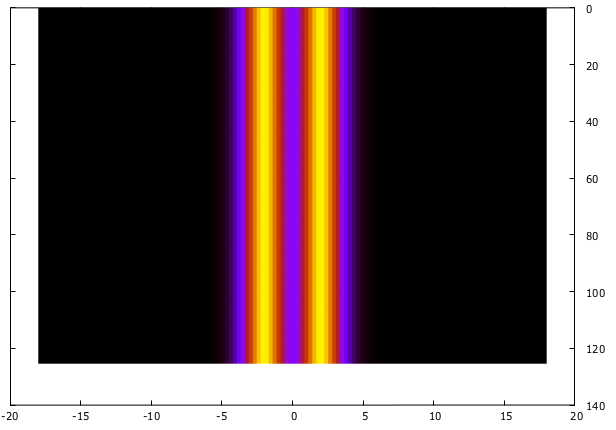
\includegraphics[width=1.2\textwidth]{img/finit_2beams.png}
        
        Initial condition
      \column{0.5\textwidth}
      	\centering
        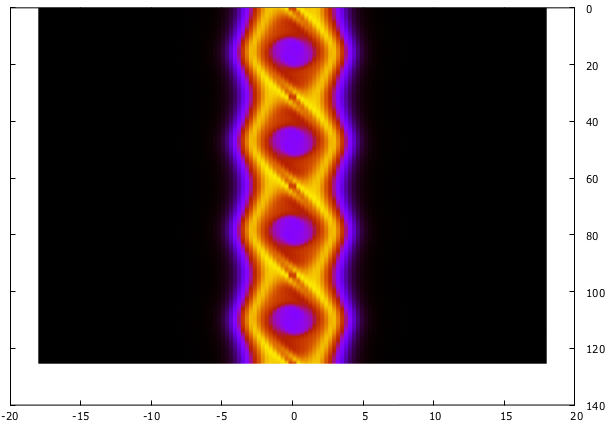
\includegraphics[width=1.2\textwidth]{img/fvp_2beams.png}
        
        Result
    \end{columns}
  \end{frame}
  \begin{frame}{Numerical test: two streams}
  	\framesubtitle{Electric energy}
  	\begin{figure}
        \centering
        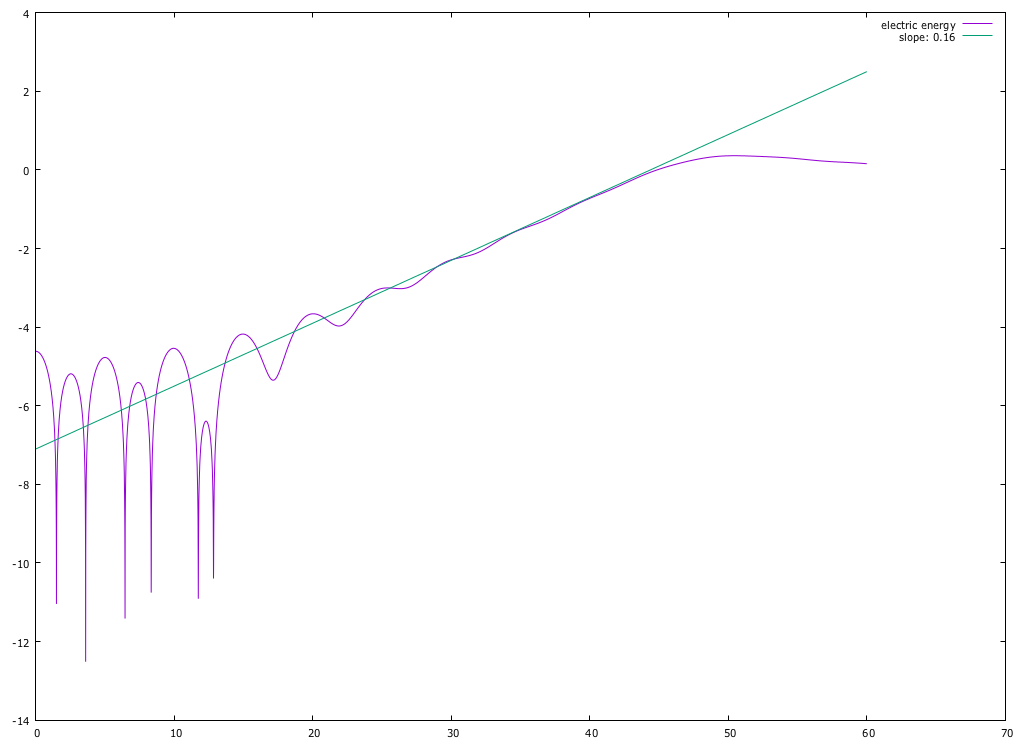
\includegraphics[height=0.55\textheight]{img/Enrj_2beams.png}
      \end{figure}
  \end{frame}


  \begin{frame}{Numerical test: Landau damping}
  	\framesubtitle{Electric energy}
  	\begin{figure}
        \centering
        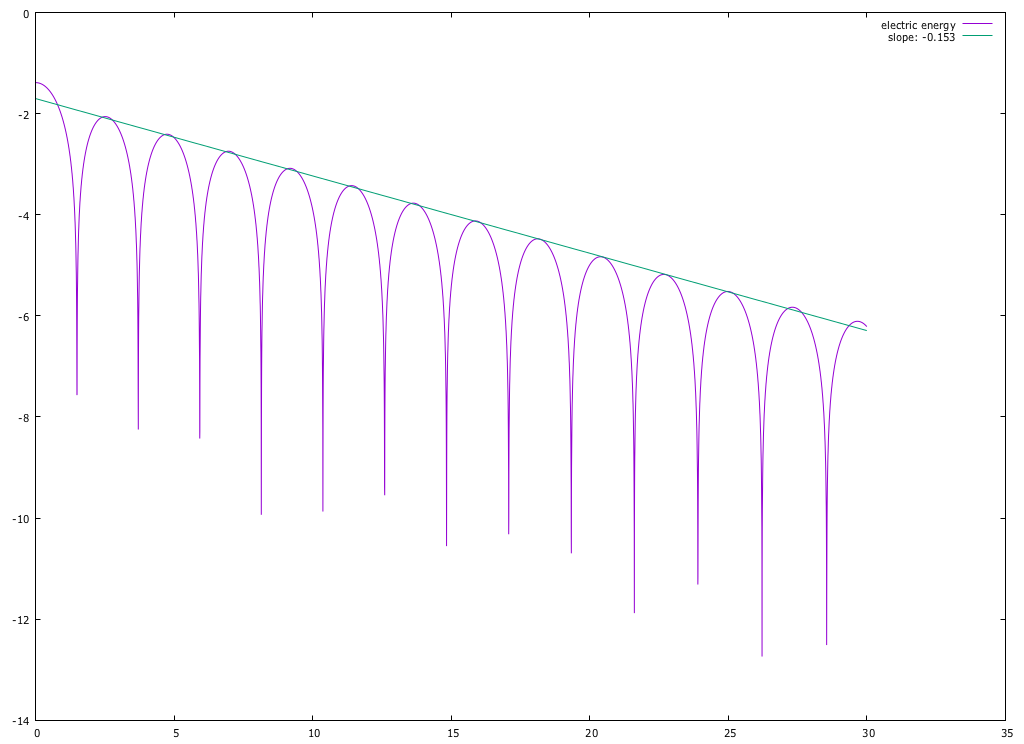
\includegraphics[height=0.55\textheight]{img/Enrj_landau.png}
      \end{figure}
  \end{frame}

  \subsection{BoT studying}
  \begin{frame}{Bump on Tail (BoT)}
  	Cold and hot particles splitting (not same as micro-macro splitting)
		$$
			f=f_c+f_h \qquad f=\mathcal{M}_{[U]}+g
		$$
		What we expect: $f_c = \mathcal{M}_{[U]}$, $f_h=g$\dots
  	\begin{figure}
        \centering
        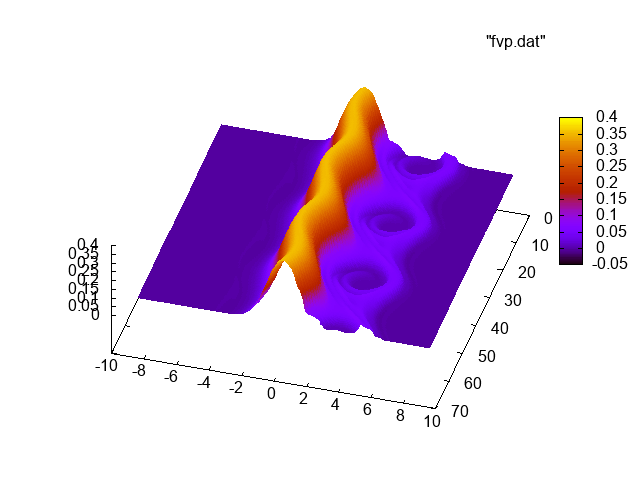
\includegraphics[height=0.65\textheight]{img/fvp_bot.png}
      \end{figure}
  \end{frame}
  \begin{frame}{BoT: $f_c$, $f_h$}
  	\begin{columns}[c]
      \column{0.5\textwidth}
        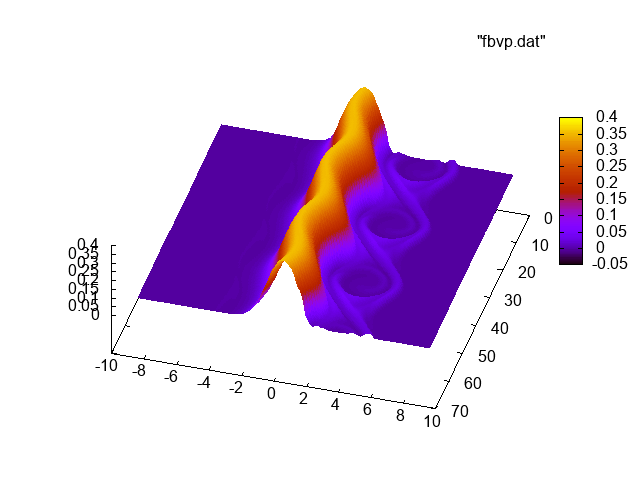
\includegraphics[width=\textwidth]{img/fbvp.png}

        $f_c$
      \column{0.5\textwidth}
        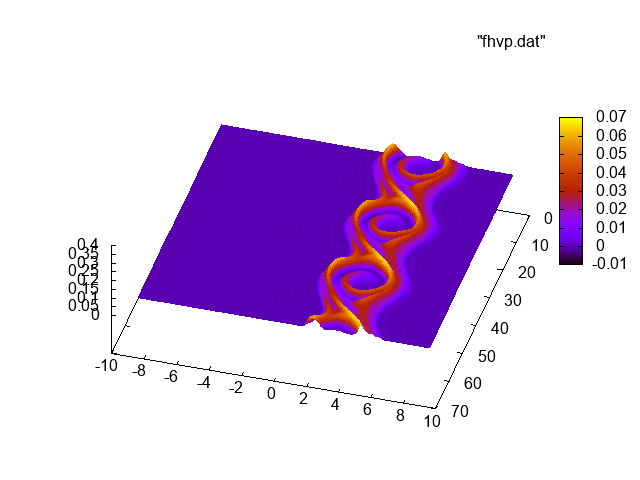
\includegraphics[width=\textwidth]{img/fhvp.png}

        $f_h$
    \end{columns}
  \end{frame}
  \begin{frame}{BoT: $f_c$ mM, $f_h$ kinetic}
  	\textbf{mM} on $f_c = \mathcal{M}_{[U_c]}+g_c$, \textbf{kinetic} on $f_h$
  	\begin{columns}[c]
      \column{0.5\textwidth}
        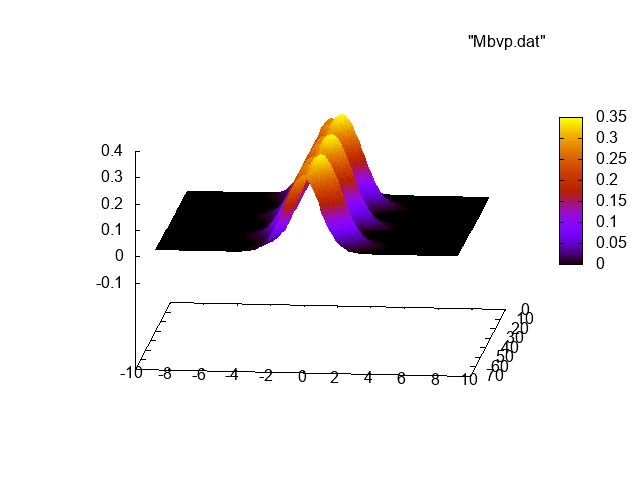
\includegraphics[width=\textwidth]{img/Mbvp_mM.png}

        $\mathcal{M}_{[U_c]}$
      \column{0.5\textwidth}
        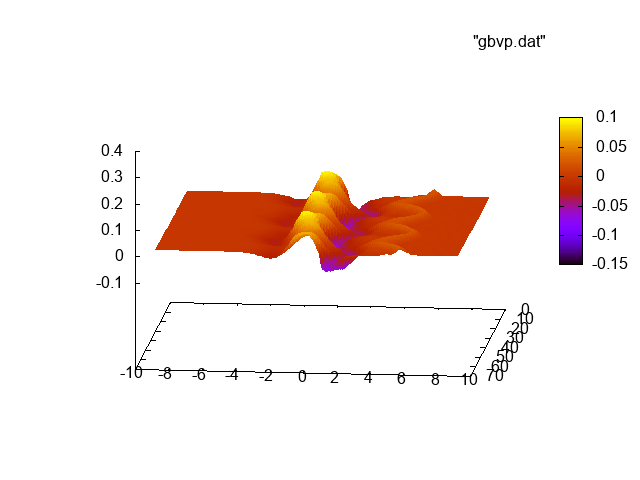
\includegraphics[width=\textwidth]{img/gbvp_mM.png}

        $g_c$
    \end{columns}
  \end{frame}
  \begin{frame}{BoT: $f_c$ mM, $f_h$ kinetic}
  	\textbf{mM} on $f_c = \mathcal{M}_{U_c}+g_c$, \textbf{kinetic} on $f_h$
  	\begin{columns}[c]
      \column{0.5\textwidth}
        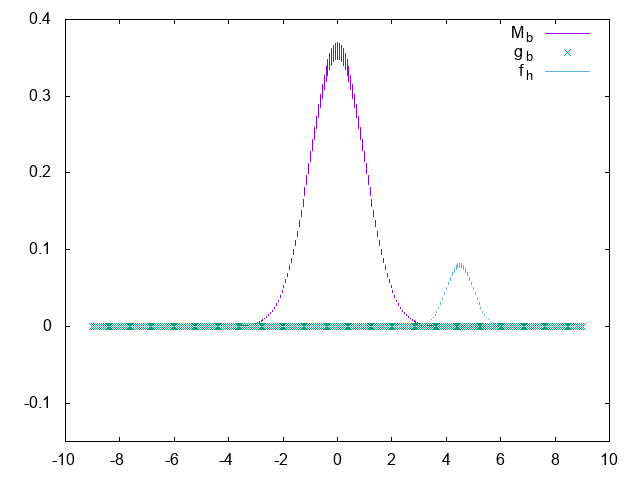
\includegraphics[width=\textwidth]{img/Mgbfhinit_coupe.png}

        Initial condition
      \column{0.5\textwidth}
        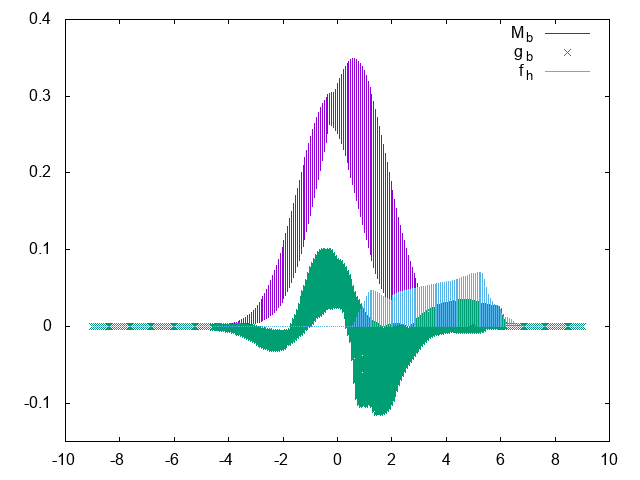
\includegraphics[width=\textwidth]{img/Mgbfhvp_coupe.png}

        Result
    \end{columns}
  \end{frame}

  \begin{frame}{BoT: $f_c$ fluid approximation}
  	approximation : $f_c = \mathcal{M}_{[U_c]}$, $g_c = 0$
		\begin{figure}
			\centering
			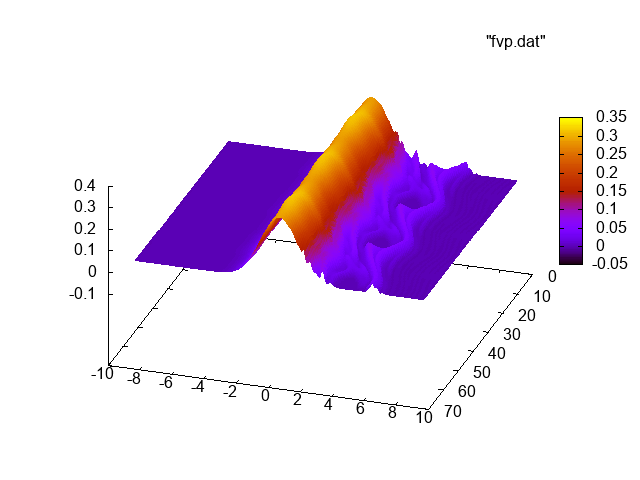
\includegraphics[height=0.8\textheight]{img/fvp_mMfluid.png}
		\end{figure}
  \end{frame}
  \begin{frame}{BoT: $f_c$ fluid approximation}
  	approximation : $f_c = \mathcal{M}_{[U_c]}$, $g_c = 0$
  	\begin{columns}[c]
      \column{0.5\textwidth}
        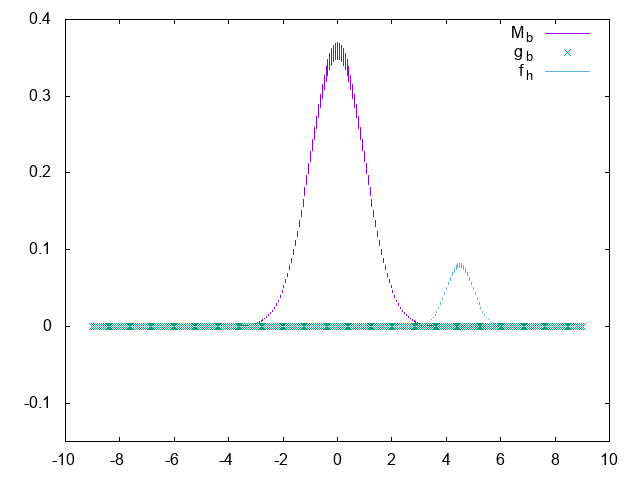
\includegraphics[width=\textwidth]{img/Mgbfhinit_coupe.png}

        Initial condition
      \column{0.5\textwidth}
        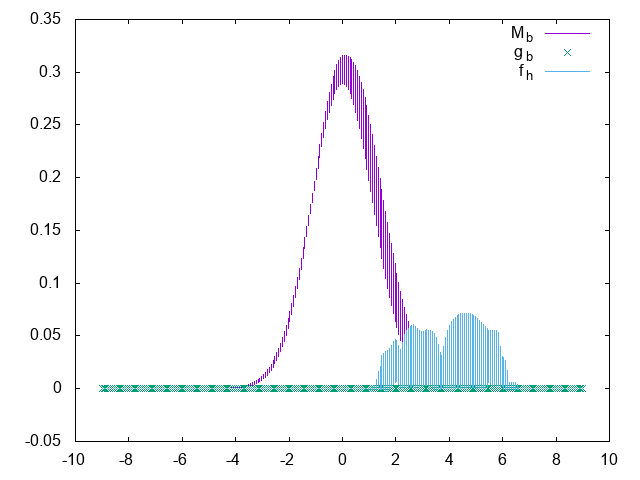
\includegraphics[width=\textwidth]{img/Mg0bfhvp_coupe.png}

        Result
    \end{columns}
  \end{frame}

  \begin{frame}{Ideas}
  	\begin{itemize}
  		\item Physicist idea (IPP Garching): $f_c = \delta_{v-u_c}$
  		\item Computer scientist idea: reduce grid in $v$ around effective data for $f_h$
  	\end{itemize}
  \end{frame}


  %%%%%%%%%%%%%%%%%%%%%%%%%%
 \section{Conclusion}
 \begin{frame}{Conclusion}
 	\begin{description}
 		\item[\cmark{}] WENO approved! \begin{itemize}
 			\item High order, no oscillation, no problem in multi-D (CFL ?)
 			\item Works well with RK3 (even with stiff term)
 			\item Could be use for Euler part
 		\end{itemize}
 	\end{description}
 \end{frame}
 \begin{frame}{Future works}
 	\begin{itemize}
		\item Still a grid in phase space for 1Dx 3Dv or 3Dx 3Dv? (MC? PIC?)
		\item Code refactoring: some optimization and adaptive grid (no global variables) (Julia? C++?)
		\item Better understanding of SSPRK(3,3) diffusion, stability of couple of time-space schemes
		\item Automatic study of different schemes (\emph{SymPy} \& \emph{NodePy})
		\item Approve approximation of $f_c$ with conservative variables, and integrate Dirac modeling
 	\end{itemize}
 \end{frame}

 \begin{frame}[plain]
  \vfill
 	{\usebeamerfont{title}Tank you for your attention}
  \vfill
 \end{frame}
\appendix



  %%%%%%%%%%%%%%%%%%%%%%%%%%
\backupbegin

  \section{Construction de la fonction $h(t,x)$}
  \begin{frame}{Discrétisation du modèle micro-macro approximé}
    Détermination \emph{a priori} de la fonction $h$ : \\

    Zone \emph{hors équilibre} au cours du temps :
    $$
      \textrm{supp}\, h(t,x) = \Omega_K(t)
    $$

    Étude du support numérique (seuil à $10^{-5}$) de $(G_{i}^n)_3$  :
    $$
      \mathscr{I}^n = \left\{ i\in [\![ 0 , N_x ]\!] , \left|{\color{dgreen} \langle vm(v)g^n \rangle_{_x=x_i} }\right| > 10^{-5} \right\}
    $$
    Étude de $g_K$ limitée à $[\![i_s^n,i_e^n]\!] = \mathscr{I}^n$
  \end{frame}

  \begin{frame}{Étude du support de $h$}
    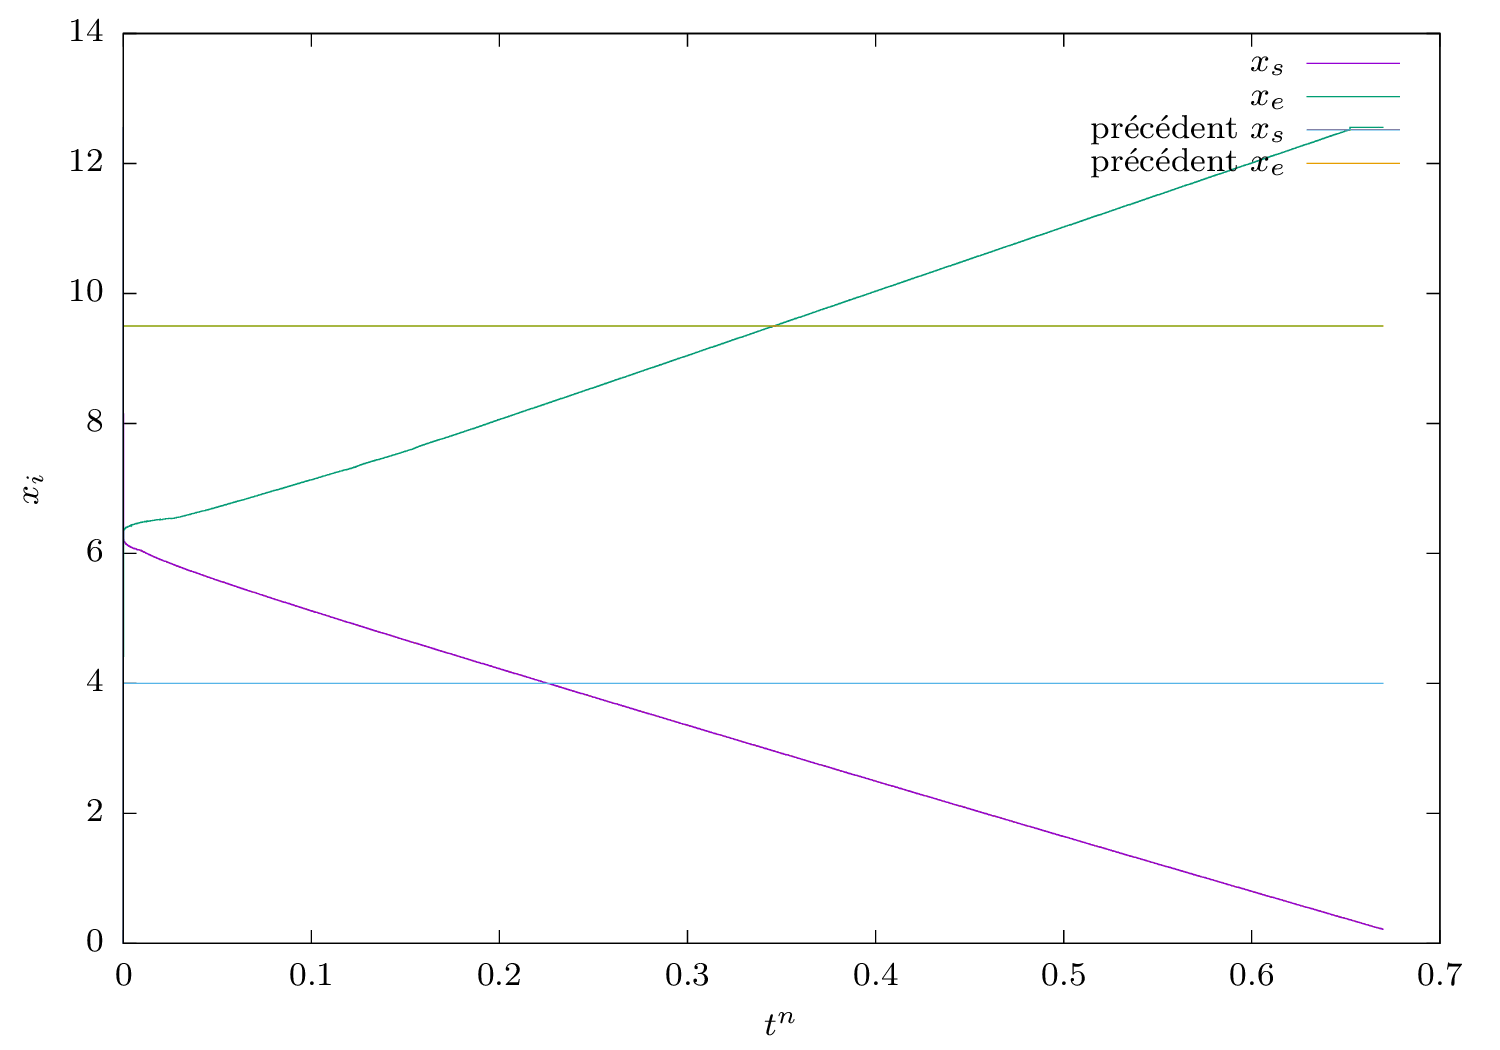
\includegraphics[width=\textwidth]{img/mimas_test/h_t/xsxe.png}
  \end{frame}

  \section{Euler's equations}
  \begin{frame}{Euler's equations}
  $$
  	\partial_t U + \nabla_x\cdot \mathcal{F}(U) = S_E(U)
	$$
  $$
  \mathcal{F}(U) = \begin{pmatrix}
    \rho u       \\
    \rho u\otimes u + p \mathbb{I}_d \\
    u(e+p)
  \end{pmatrix} \qquad S(U) = \begin{pmatrix} 0 \\ \rho E \\ 2\rho uE \end{pmatrix}
	$$
	pressure: $p = 2(e - \frac{1}{2}\rho |u|^2)$

  \end{frame}
  \section{WENO scheme}
  \begin{frame}{WENO scheme}
  Model:
	$$
	  \partial_t u + \partial_x(a u) = 0
	$$

	We would approximate $\partial_x(au)_{|x=x_i,v=v_k}$:
	$$
	  \partial(au)_{|x=x_i,v=v_k} \approx \frac{1}{\Delta x}(\hat{u}_{i+\frac{1}{2},k} - \hat{u}_{i-\frac{1}{2},k})
	$$

  \end{frame}
  \begin{frame}{WENO flux}
	$$
	  \begin{aligned}
	    \hat{u}_{i+\frac{1}{2},k}^+ =\,&w_0^+\left(\frac{2}{6}u_{i-2,k}^+ - \frac{7}{6}u_{i-1,k}^+ + \frac{11}{6}u_{i,k}^+\right) \\
	                        +\,&w_1^+\left(-\frac{1}{6}u_{i-1,k}^+ + \frac{5}{6}u_{i,k}^+   +  \frac{2}{6}u_{i+1,k}^+\right) \\
	                        +\,&w_2^+\left( \frac{2}{6}u_{i,k}^+   + \frac{5}{6}u_{i+1,k}^+ -  \frac{1}{6}u_{i+2,k}^+\right)
	  \end{aligned}
	$$
	and
	$$
	  \begin{aligned}
	  \hat{u}_{i+\frac{1}{2},k}^- =\,&w_2^-\left(-\frac{1}{6}u_{i-1,k}^- + \frac{5}{6}u_{i,k}^-   + \frac{2}{6}u_{i+1,k}^-\right) \\
	                        +\,&w_1^-\left( \frac{2}{6}u_{i,k}^-   + \frac{5}{6}u_{i+1,k}^- - \frac{1}{6}u_{i+2,k}^-\right) \\
	                        +\,&w_0^-\left(\frac{11}{6}u_{i+1,k}^- - \frac{7}{6}u_{i+2,k}^- + \frac{2}{6}u_{i+3,k}^-\right)
	  \end{aligned}
	$$
  \end{frame}
  \begin{frame}{WENO weights}
	$$
	  w_{n}^{\pm} = \frac{\tilde{w}_{n}^{\pm}}{\sum_{m=0}^2 \tilde{w}_{m}^{\pm} } \,, \quad \tilde{w}_{n}^{\pm} = \frac{\gamma_n}{(\epsilon + \beta_{n}^{\pm})^2}
	$$

	$$
	  \gamma_{0} = \frac{1}{10} \,, \quad \gamma_{1} = \frac{3}{5}\,,\quad \gamma_{2} = \frac{3}{10}
	$$

	$\epsilon = 10^{-6}$ numerical value to prevent the denominator from being $0$
  \end{frame}
  \begin{frame}{WENO Indicator of Smoothness}
	$$
	 \begin{aligned}
	   \beta_0^+ &= \frac{13}{12}(u^+_{i-2,k} -2u^+_{i-1,k} + u^+_{i  ,k})^2 + \frac{1}{4}( u^+_{i-2,k} - 4u^+_{i-1,k} + 3u^+_{i,k})^2 \\
	   \beta_1^+ &= \frac{13}{12}(u^+_{i-1,k} -2u^+_{i  ,k} + u^+_{i+1,k})^2 + \frac{1}{4}( u^+_{i-1,k} -  u^+_{i+1,k})^2 \\
	   \beta_2^+ &= \frac{13}{12}(u^+_{i  ,k} -2u^+_{i+1,k} + u^+_{i+2,k})^2 + \frac{1}{4}(3u^+_{i  ,k} - 4u^+_{i+1,k} + u^+_{i+2,k} )^2 
	 \end{aligned}
	$$
	and
	$$
	 \begin{aligned}
	   \beta_0^- &= \frac{13}{12}(u^-_{i+1,k} -2u^-_{i+2,k} + u^-_{i+3,k})^2 + \frac{1}{4}(3u^-_{i+1,k} - 4u^-_{i+2,k} + u^-_{i+3,k})^2 \\
	   \beta_1^- &= \frac{13}{12}(u^-_{i  ,k} -2u^-_{i+1,k} + u^-_{i+2,k})^2 + \frac{1}{4}(u^-_{i,k} - u^-_{i+2,k})^2 \\
	   \beta_2^- &= \frac{13}{12}(u^-_{i-1,k} -2u^-_{i  ,k} + u^-_{i+1,k})^2 + \frac{1}{4}(u^-_{i,k} - 4u^-_{i,k} + 3u^-_{i+1,k})^2
	 \end{aligned}
	$$
  \end{frame}

 \backupend
\end{document}